\section{Phase Shift}
\subsection{Finite Range Potentials}\label{finite_range_potentials}

Physicists learn a lot from scattering experiments. In fact, Rutherford first learned about the structure of the atom by scattering alpha particles (helium nuclei) off thin layers of gold. We have \textbf{elastic scattering} if particles do not change type; this typically exists for low energies. At high energies, scattering becomes quite complicated due to the creation of new particles.

The scattering of a particle off a fixed target is studied by working with a particle moving in a potential $V(x)$ created by the target. Even in the case of collisions, it is generally possible to study the problem using center of mass coordinates and considering scattering in a potential.

We consider elastic scattering in the general potential in Figure \ref{general_potential}.

\begin{figure}
    \centering
    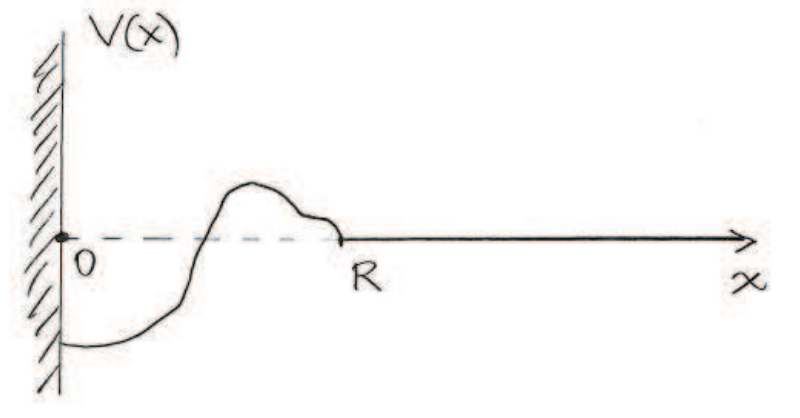
\includegraphics[width=0.5\linewidth]{resources/images/general_potential.png}
    \caption{A general potential $V(x)$.}
    \label{general_potential}
\end{figure}

This potential is given by $$V(x)=\begin{cases}\infty & x<0 \\V'(x) & 0<x<R \\ 0 & x>R\end{cases}$$We call this a \textbf{finite range potential}, because the nontrivial part of the potential $V'(x)$ exists only for a finite range $R$ from the origin. Furthermore, everything happens in $x>0$ because of an infinite wall at $x=0$. We imagine sending in incident waves from the right and analyzing the reflected waves. 

Consider first the case where $V'(x)=0$, so that $$V(x)=\begin{cases} 0 & x>0 \\ \infty & x\leq 0 \end{cases}$$ We have a free particle constrained to the positive real line. The solutions can be constructed using a linear combination of momentum eigenstates $e^{\pm ikx}$ where $$k^2=\frac{2mE}{\hbar^2}.$$Even better, we can divide this solution by $2i$ to find $$\boxed{\phi(x)=-\frac{e^{-ikx}}{2i}+\frac{e^{ikx}}{2i}=\sin kx.}$$The incoming wave is $-\frac{e^{-ikx}}{2i}$ and the reflected wave is $\frac{e^{ikx}}{2i}$. Both carry the same amount of probability current, so current conservation is satisfied. 

We now consider the more interesting case when $V'(x)\neq 0$. This potential still acts over a finite range $0<x<R$, and we will eventually be interested in computing the energy eigenstate wavefunction $\psi(x)$ in this region. However, we can first consider $\psi(x)$ *outside* the range of the potential. We will take the incoming wave to be the same as before: $$\text{Incoming wave:}\quad -\frac{e^{-ikx}}{2i}.$$The outgoing wave must have the same energy as the incident wave, so it must also have an $e^{ikx}$ factor: $$\psi(x)=-\frac{e^{-ikx}}{2i}+A\frac{e^{ikx}}{2i}.$$Note that $A$ cannot depend on $x$, since that would change the momentum of the outgoing wave. Furthermore, we found in Section \ref{energy_above_barrier} that the probability current of $Ae^{-ikx}+Be^{ikx}$ is proportional to $|A|^2-|B|^2$, so the only constant that we can attach to the outgoing wave is a pure phase $$A=e^{2i\delta(k)}.$$A natural range of $\delta$ would be from $0$ to $2\pi$, but it will turn out to be easier to let it range through all of $\mathbb{R}$ in order to get a \textit{continuous} function of $k$. 

Adding the incident and reflected waves, we get $$\psi(x)=\frac{1}{2i}(-e^{-ikx}+e^{ikx+2i\delta})=e^{i\delta}\frac{1}{2i}(-e^{-ikx-i\delta}+e^{ikx+i\delta}).$$Notably, this is equivalent to $$\boxed{\psi(x)=e^{i\delta}\sin (kx+\delta),\quad x>R.}$$

\subsection{Scattered Waves}\label{scattered_waves}

We consider the probability amplitudes of the solutions in the cases when $V'(x)=0$ and when $V'(x)\neq 0$. We have \begin{align*}|\phi(x)|^2&=\sin^2(kx),\\|\psi(x)|^2&=\sin^2(kx+\delta)\end{align*}Notice, therefore, that for any feature of $\phi(x)$ that we might find at some position $x_0$, we will find the same feature in $\psi(x)$ at $x=x_0-\frac{\delta}{k}$. This is depicted in Figure \ref{phase_shift_scattered_wave}. For $\delta>0$, the wave is ``pulled in'' by an amount $\delta/k$, and the potential is attractive. For $\delta<0$, the wave is ``pushed out'' by the same amount, and the potential is repulsive.

\begin{figure}
    \centering
    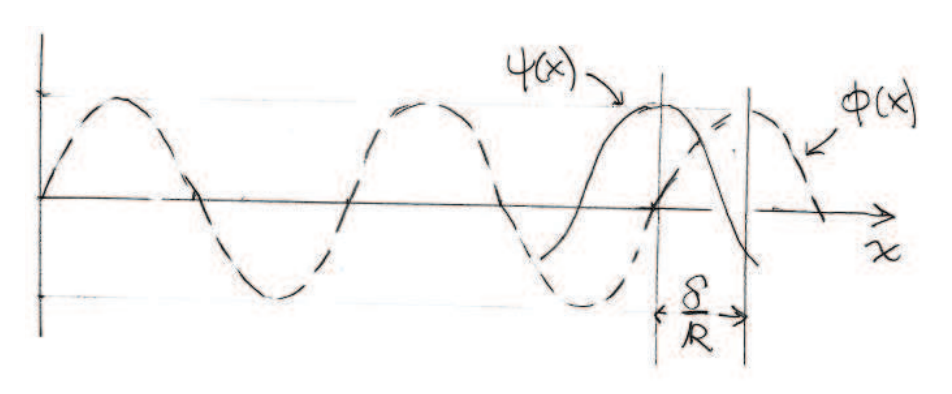
\includegraphics[width=0.5\linewidth]{resources/images/phase_shift_scattered_wave.png}
    \caption{The wave in the case of a nonzero potential is shifted by a distance $\frac{\delta}{k}$.}
    \label{phase_shift_scattered_wave}
\end{figure}

We define the \textbf{scattered wave} $\psi_s(x)$ as the extra wave in the solution $\psi(x)$ that would vanish for the case of zero potential. That is, we define $\psi_s(x)$ such that $$\psi(x)=\phi(x)+\psi_s(x).$$Recall that $\phi$ and $\psi$ have the same incident wave, so $\psi_s$ must be an outgoing wave. Indeed, we find $$\psi_s(x)=\psi(x)-\phi(x)=\frac{1}{2i}(-e^{-ikx}+e^{ikx+2i\delta}+e^{-ikx}-e^{ikx})=\frac{1}{2i}(e^{ikx+2\delta}-e^{ikx}).$$Factoring, we get $$\psi_s(x)=e^{i\delta}e^{ikx}\frac{1}{2i}(e^{i\delta}-e^{-i\delta})=e^{i\delta}\sin(\delta)e^{ikx}=A_se^{ikx},$$with $A_s=e^{i\delta}\sin\delta$. We call $A_s$ the \textbf{scattering amplitude}, since it is the amplitude of the scattered wave $\psi_s$. While these states cannot be normalized, the probability to scatter will be given by $$|A_s|^2=\sin^2\delta.$$

\subsection{Time Delay}\label{time_delay}

Consider an incident wavepacket given for $x>R$ by $$\psi_{inc}(x>R,t)=\int_0^\infty dk\,f(k)e^{-ikx}e^{-iE(k)t/\hbar},$$where $f(k)$ is a real function peaked around $k=k_0$. We find the reflected wavepacket by noting that $\psi_{inc}$ is a superposition of incident waves, so the reflection must be the associated superposition of reflected waves. We see that $$\psi_{ref}(x>R,t)=-\int_0^\infty dk\,f(k)e^{ikx}e^{2i\delta(k)}e^{-iE(k)t/\hbar}.$$We now use the stationary phase approximation to find the motion of the peak of the wavepacket. Recall that we must have a stationary phase when $k=k_0$. For the incident wave, we get that $$x=-\frac{\hbar k_0}{m}t=-v_gt,$$where $v_g$ is the group velocity. This makes sense; the peak of the incident wavepacket simply moves to the left with constant velocity. 

On the other hand, for the reflected wave, we get $$x=v_g\bigg(t-2\hbar\delta'(E(k_0))\bigg).$$Here we see the time delay $\Delta t=2\hbar\delta'(E)$, as stated in Section \ref{wavepackets_energy_below_barrier}. We can compare this delay to a natural time in the problem. We first write $$\Delta t=2\hbar\frac{dk}{dE}\frac{d\delta}{dk}=\frac{2}{(\frac{1}{\hbar}\frac{dE}{dk})}\frac{d\delta}{dk}=\frac{2}{(\frac{d\omega}{dk})}\frac{d\delta}{dk}=\frac{2}{v_g}\frac{d\delta}{dk}.$$Multiplying by $\frac{1}{R}$, we get that $$\frac{1}{R}\frac{d\delta}{dk}=\frac{\Delta t}{(\frac{2R}{v_g})}=\frac{\text{delay}}{\text{free transit time}}.$$Note that the right-hand side is the ratio of the time delay to the time it would take a free particle to travel in and out of the range of the potential.

\begin{framedexpl}[Phase shift for a potential well]
    Find the energy eigenstates of the potential in Figure \ref{phase_shift_potential_well} given by $$V(x)=\begin{cases} -V_0 & 0<x<a \\ 0 & x>a \\ \infty & x<0 \end{cases}$$
\end{framedexpl}

\begin{figure}[H]
    \centering
    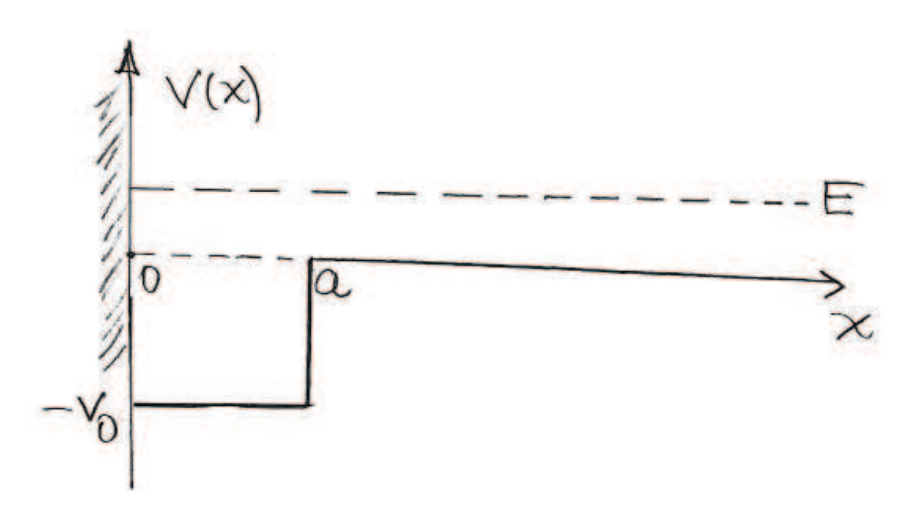
\includegraphics[width=0.5\linewidth]{resources/images/phase_shift_potential_well.png}
    \caption{A potential well with width $a$ and depth $V_0$.}
    \label{phase_shift_potential_well}
\end{figure}

\begin{framedansw}
    We found in Section \ref{finite_range_potentials} that the solution outside the well is of the form $e^{i\delta}\sin(kx+\delta)$. Inside the well, the boundary condition $\psi(0)=0$ forces the solution to be a sine, giving us $$\psi(x)=\begin{cases}e^{i\delta}\sin(kx+\delta) & x>a \\ A\sin(k'x) & 0<x<a\end{cases}$$where $$k^2=\frac{2mE}{\hbar^2},\quad k'^2=\frac{2m(E+V_0)}{\hbar^2}.$$The boundary conditions at $x=a$ give \begin{align*}A\sin(k'a)&=e^{i\delta}\sin(ka+\delta), \\ k'A\cos(k'a) &= ke^{i\delta}\cos(ka+\delta).\end{align*}Dividing the second equation by the first, we have $$k\cot(ka+\delta)=k'\cot(k'a).$$We now use the identity $$\cot(A+B)=\frac{\cot A\cot B-1}{\cot A+\cot B},$$which gives us $$\frac{k'}{k}\cot(k'a)=\cot(ka+\delta)=\frac{\cot(ka)\cot(\delta)-1}{\cot(ka)+\cot(\delta)}.$$Solving this equation for $\delta$ yields $$\boxed{\cot\delta=\frac{\tan(ka)+\frac{k'}{k}\cot(k'a)}{1-\frac{k'}{k}\cot(k'a)\tan(ka)}}.$$
    As usual, we characterize the well by the unit-free constant $$z_0=\frac{2mV_0a^2}{\hbar^2}.$$We also have$$(k'a)^2=z_0^2+(ka)^2.$$Using this relation, and letting $ka=u$, we can solve for $\delta$ solely in terms of the unit-free constants $u$ and $z_0$: $$\tan\delta=\frac{1-\sqrt{1+(z_0/u)^2}\cot(\sqrt{z_0^2+u^2})\tan u}{\tan u+\sqrt{1+(z_0/u)^2}\cot(\sqrt{z_0^2+u^2})}.$$

\end{framedansw}

\begin{framedrmk*}[Messy formulas]
    When dealing with phase shifts, many of the resulting formulas will seem forbiddingly complicated, even when simplified as far as possible. Remember that it is always possible to plot such a formula with a computer for various values of $V_0$.
\end{framedrmk*}

\subsection{Excursion of the Phase Shift}

Figure \ref{phase_shift_plots} shows the phase shift $\delta$, the scattering probability $\sin^2\delta$, the time delay $\frac{1}{a}\frac{d\delta}{dk}$, and the wavefunction amplitude $A$ inside the well as functions of $u=ka$, a unit-free proxy for the energy, for $z_0=0.59\pi$.

\begin{figure}
    \centering
    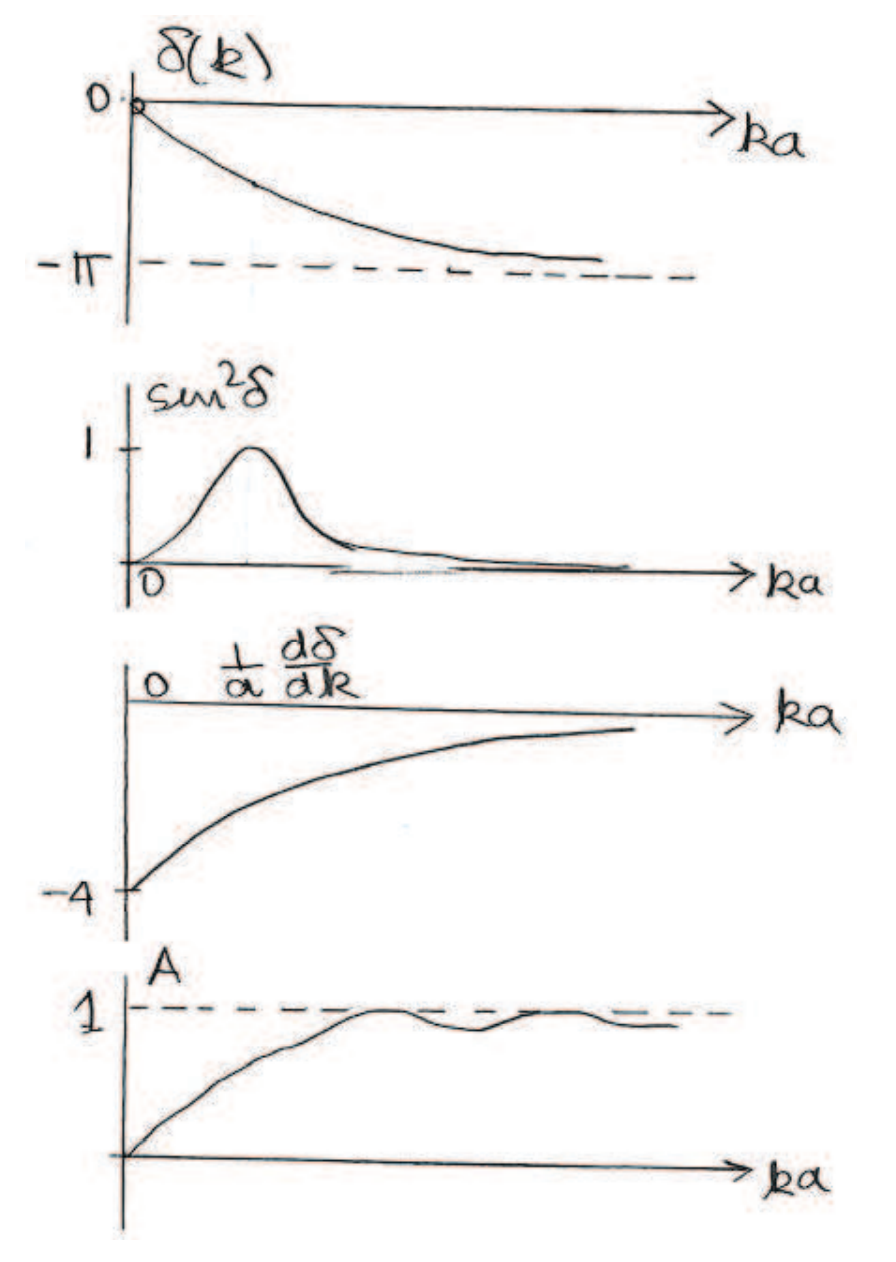
\includegraphics[width=0.45\linewidth]{resources/images/phase_shift_plots.png}
    \caption{Four plots for the potential well with $z_0=0.59\pi$.}
    \label{phase_shift_plots}
\end{figure}

Note that the phase $\delta$ begins at $0$ for $0$ energy and approaches $-\pi$ for infinite energy. The \textbf{phase excursion} is thus $\pi$. In the next section, we will prove a relationship between the phase excursion and the number of bound states of the potential. Since $z_0$ is in the range $(\frac{\pi}{2},\pi)$, the half-square well with this value of $z_0$ has one bound state.

The value of $|A_s|^2=\sin^2\delta$ represents the probability of scattering and peaks for the value of $ka$ for which $|\delta|=\pi/2$.

Next we have the unit-free time delay $\frac{1}{a}\frac{d\delta}{dk}$. Note that the delay is always negative. This is because as the particle moves over the well, its kinetic energy increases by $V_0$, so it speeds up.

Finally, the last plot shows the magnitude $A$ of the constant that gives the amplitude of the wavefunction within the well. This is identical to Figure \ref{resonant_transmission_example}.

At very large energy, the particle barely notices the potential; the phase shift approaches $-\pi$, which is equivalent to approaching $0$ and having no phase shift. Accordingly, $|A_s|^2$ approaches $0$, so no scattering occurs, and the time delay also approaches $0$. Finally, $A\to 1$, so the amplitude of the wavefunction is unaffected by the well.

\subsection{Levinson's Theorem}

We now reach one of the most challenging and counterintuitive results in this course. \textbf{Levinson's theorem} relates the number of bound states of a potential to the excursion of the phase shift as energy ranges from $0$ to $\infty$.

\begin{framedthm}[Levinson's theorem]
    The number $N_b$ of bound states of a potential is related to the excursion of the phase shift $\delta(E)$ by the relation $$\boxed{N_b=\frac{1}{\pi}\bigg(\delta(0)-\delta(\infty)\bigg).}$$
\end{framedthm}

\begin{proof}
    Consider an arbitrary potential $V(x)$ of range $R$, with an infinite wall at $x=0$ (shown to the left in Figure \ref{regulator}). This potential has a finite number of bound states. However, the scattering states belong to a continuum and are uncountable. To be able to count all the states, we place another infinite wall at $x=L$, thus discretizing the scattering states and making them countable. We call this second wall the \textbf{regulator}, and the new potential (shown to the right) the \textbf{regulated potential}. Of course, the spectrum will be different for the regulated potential, but these changes become negligible as $L$ goes to infinity.

    The key of the proof will be to compare counting the states in the regulated potential to those in the $V=0$ potential, also regulated with a wall at $x=L$. Consider the positive energy eigenstates of the regulated $V=0$ potential. These correspond to the wavefunctions $\phi(x)=\sin kx$, with the second wall requiring $\phi(L)=0$. We thus have $$kL=n\pi,\quad n\in\mathbb{N}.$$The values of $k$ have been quantized. Let $dk$ be an infinitesimal interval in wavenumber with $dn$ the number of states within in the interval when $V=0$. We have $$dn=\frac{L}{\pi}dk.$$
    
    Recall that when $V(x)$ is an arbitrary finite-range potential, the solutions for $x>R$ -- all of which are positive-energy solutions -- have the form $$\psi(x)=e^{i\delta}\sin(kx+\delta).$$The boundary condition $\psi(L)=0$ due to the regulator implies the quantization $$kL+\delta(k)=n'\pi,\quad n'\in\mathbb{Z}.$$We again differentiate to determine the number of positive-energy states $dn'$ within the infinitesimal interval $dk$ in wavenumber: $$dn'=\frac{L}{k}dk+\frac{1}{\pi}(\frac{d\delta}{dk})dk.$$Imagine slowly deforming the initial $V=0$ potential to get to the potential $V$. Notice that in this process, we lose some number of positive-energy solutions in the interval $dk$, given by $$dn-dn'=-\frac{1}{\pi}(\frac{d\delta}{dk}dk).$$The total number of positive energy solutions lost as the potential $V$ is turned on given by integrating the above result over the full range of $k$: $$\text{lost positive-energy solutions}=-\int_0^\infty\frac{1}{\pi}\frac{d\delta}{dk}dk=-\frac{1}{\pi}(\delta(\infty)-\delta(0)).$$However, in the process of slowly deforming the potential, states do not disappear. Therefore, the lost positive-energy states must now appear as \textit{negative-energy states}, or bound states! This process is depicted in Figure \ref{levinson_diagram}. Letting $N_b$ denote the number of bound states in the new potential $V$, we arrive at our intended result $$N_b=\frac{1}{\pi}(\delta(0)-\delta(\infty)).$$
\end{proof}

\begin{figure}
    \centering
    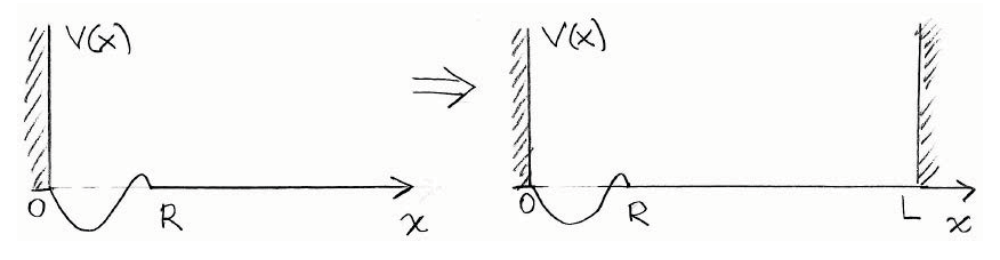
\includegraphics[width=0.5\linewidth]{resources/images/regulator.png}
    \caption{An arbitrary potential $V(x)$ (left) and the regulated potential (right).}
    \label{regulator}
\end{figure}

\begin{figure}
    \centering
    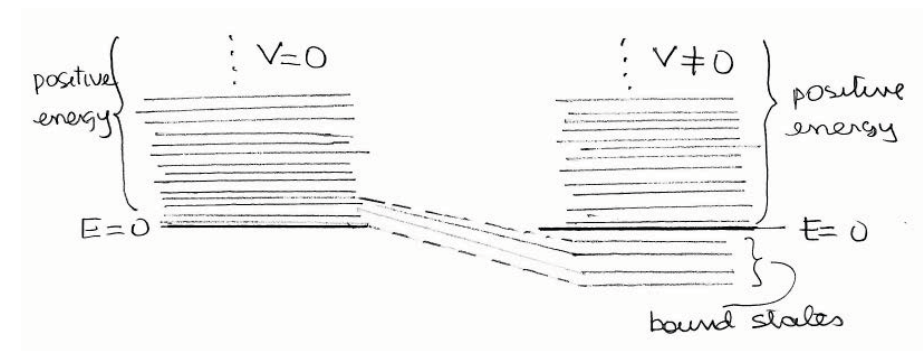
\includegraphics[width=0.5\linewidth]{resources/images/levinson_diagram.png}
    \caption{As $V$ is turned on, some positive-energy states are lost, instead becoming negative-energy bound states.}
    \label{levinson_diagram}
\end{figure}

\section{Resonance}
\subsection{Arbitrary Time Delay}

We have previously found the time delay $\Delta t=2\hbar\delta'(E)$ associated with the reflected wavepacket that emerges from a finite-range potential. If the time delay is negative, the reflected wave emerges ahead of time, and if the time delay is positive, the reflected wave emerges late. We introduce the subject of resonances by asking the following question.

\begin{framedquest*}
    Can we get an arbitrarily large negative time decay?
\end{framedquest*}

The answer is no. If the time delay was sufficiently large, it would violate causality: the incoming packet would be reflected even before it reached the potential, which is impossible. In fact, the largest possible negative time delay should be as if we had perfect reflection when the incoming packet hit $x=R$.\footnote{This argument seems solid, but there are actually some subtle quantum corrections for the largest possible negative time delay. Luckily, these vanish for packets with large energy, and our final constraint is quite accurate.} In this case, the time delay would be $-\frac{2R}{v_0}$, where the packet has velocity $v_0$. Thus, we expect $$\Delta t=2\hbar\frac{d\delta}{dE}\geq -\frac{2R}{v_0}.$$This can be simplified a bit: $$2\hbar\frac{1}{\frac{dE}{dk}}\frac{d\delta}{dk}=2\hbar\frac{1}{\hbar v_0}\frac{d\delta}{dk}\geq -\frac{2R}{v_0},$$which produces the constraint $$\frac{d\delta}{dk}\geq -R.$$  

We can also ask the opposite question.

\begin{framedquest*}
    Can we get an arbitrarily large positive time delay?
\end{framedquest*}

The answer is yes! This can happen if the wavepacket gets temporarily trapped in the potential, in which case we expect the probability amplitude to become extremely large in the $0<x<R$ region. If the wavepacket is trapped for a long time, we have a \textbf{resonance}. The state is a bit like a bound state in that it gets localized in the potential, at least for a while. We can achieve this with the potential $$V(x)=\begin{cases}\infty & x\leq 0 \\ -V_0 & 0<x<a \\ V_1 & a<x<2a \\ 0 & x>2a\end{cases}$$This potential is shown in Figure \ref{resonant_potential}. The particle gets trapped for a long time in the well from $x=0$ to $x=a$, but it has some small probability of leaking through the $V_1$ barrier. 

\begin{figure}
    \centering
    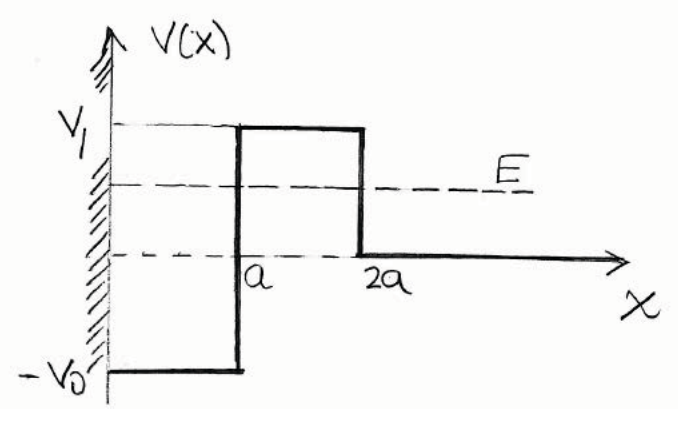
\includegraphics[width=0.5\linewidth]{resources/images/resonant_potential.png}
    \caption{A potential well with a barrier.}
    \label{resonant_potential}
\end{figure}

We search for resonances with energies in the range $0<E<V_1$; this is the range for which we may have an incoming wave in the $x>2a$ region but not in the $a<x<2a$ region. 

We define $$k^2=\frac{2mE}{\hbar^2},\quad k'^2=\frac{2m(E+V_0)}{\hbar^2},\quad \kappa^2=\frac{2m(V_1-E)}{\hbar^2}.$$In the region $0<x<a$ we use trigonometric functions of $k'x$. In the region $a<x<2a$ we use hyperbolic functions of $\kappa a$. Finally, in the region $x>2a$ we use the canonical solution $\psi(x)=e^{i\delta}\sin(kx+\delta)$.

Since $\psi(0)=0$, we must have a sine function in the first region. The solution in the second region can be written as a linear combination of $\cosh\kappa(x-a)$ and $\sinh\kappa(x-a)$, which we choose in order to force continuity at $x=a$: $$\psi(x)=\begin{cases}A\sin(k'x) & 0<x<a \\ A\sin(k'a)\cosh\kappa(x-a)+B\sinh\kappa(x-a) & a<x<2a\\ e^{i\delta}\sin(kx+\delta) & x>2a\end{cases}$$

After implementing the remaining boundary conditions, we can solve for the phase shift $\delta$. The final answer is $$\tan(2ka+\delta)=\frac{ka}{\kappa a}\frac{\sin(k'a)\cosh(\kappa a)+\frac{k'}{k}\cos(k'a)\sinh(\kappa a)}{\sin(k'a)\sinh(\kappa a)+\frac{k'}{\kappa}\cos(k'a)\cosh(\kappa a)}.$$

This expression is very complicated, so it's best to use a computer to do numerical work. For this we define $$z_0^2=\frac{2mV_0a^2}{\hbar^2},\quad z_1^2=\frac{2mV_1a^2}{\hbar^2},\quad u=ka.$$Then we can express both $k'a$ and $\kappa a$ as functions of these unit-free constants: $$(k'a)^2=z_0^2+u^2,\quad (\kappa a)^2=z_1^2-u^2.$$We also let $e=\frac{E}{V_1}$ be a unit-free proxy for the energy, so that $$e=\frac{E}{V_1}=\frac{\hbar^2k^2a^2}{2mV_1a^2}=\frac{u^2}{z_1^2}.$$

\subsection{Example of a Resonance}\label{resonance_example}

We are now ready to make some plots. In Figure \ref{resonance_plots}, we show results for $z_0^2=1$ and $z_1^2=5$ (since $e<1$, this constrains $u<\sqrt{5}$).

\begin{figure}
    \centering
    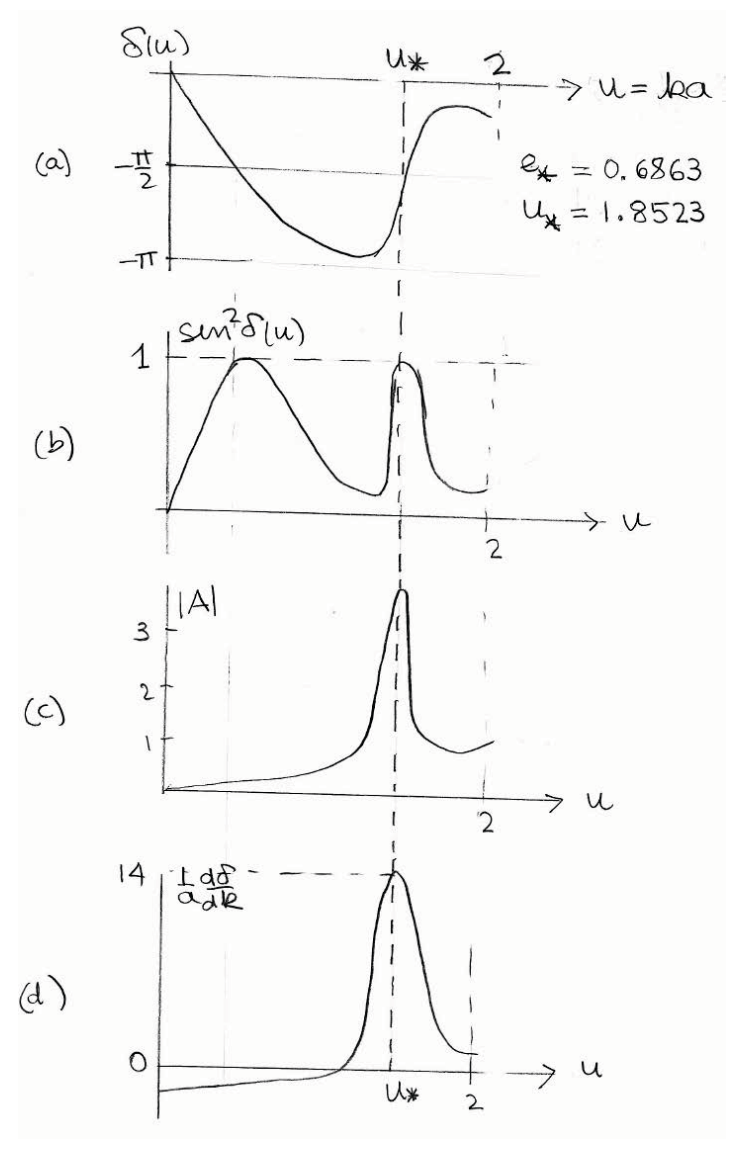
\includegraphics[width=0.4\linewidth]{resources/images/resonance_plots.png}
    \caption{Four plots for the potential with $z_0^2=1$ and $z_1^2=5$.}
    \label{resonance_plots}
\end{figure}

In part (a) of the figure, we see that $\delta(ka)$ begins by decreasing linearly, indicating a negative time delay. This is due to the low-energy waves reflecting at $x=2a$ off the $V_1$ barrier. However, as $u$ approaches $u_* \approx 1.8523$, $\delta$ increases rapidly from $\approx -\pi$ to $\approx 0$. In fact, we get a resonance at $u_*$, indicated by the peaks in the amplitude within the well in part (c) and the unit-free time delay in part (d). At $u_*$, this time delay reaches a value of about 14, meaning the delay is 14 times the free transit time $4a/v_0$!

\subsection{Modeling a Resonance}\label{modeling_a_resonance}

We've now seen an example of a resonance, but how do we find resonances formulaically? Suppose there exists a resonance at $k=\alpha$. We claim that this can be achieved by the function $$\tan\delta=\frac{\beta}{\alpha-k}.$$The plots of $\frac{\beta}{\alpha-k}$ and the arctangent of this quantity are shown in Figure \ref{resonance_modeling}. Note that the argument varies quickly in the region $(\alpha-\beta,\alpha+\beta)$. To have a resonance, we must have a sharp increase in $\delta$. Thus, the width of this region must be small, i.e. we must have $\beta\ll\alpha$.

\begin{figure}
    \centering
    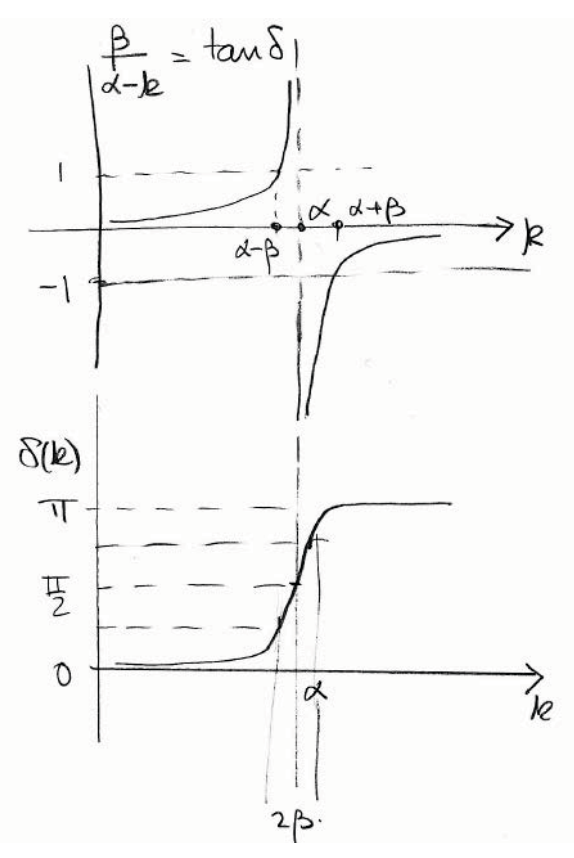
\includegraphics[width=0.4\linewidth]{resources/images/resonance_modeling.png}
    \caption{Plots of $\tan\delta$ and $\delta(k)$.}
    \label{resonance_modeling}
\end{figure}

We can also calculate $$\frac{d\delta}{dk}\bigg|_{k=\alpha}=\frac{1}{\beta},\quad|\psi_s|^2=\sin^2\delta=\frac{\beta^2}{\beta^2+(\alpha-k)^2}.$$The first result indicates that the time delay is inversely proportional to $\beta$ -- thus, resonance does indeed require small $\beta$, as reasoned above. The second gives the scattering amplitude as a function of $k$, with a peak at $k=\alpha$. This equation is most famously expressed in terms of *energy*, not momentum. Note that $$E-E_\alpha=\frac{\hbar^2}{2m}(k^2-\alpha^2)=\frac{\hbar^2}{2m}(k+\alpha)(k-\alpha).$$For $k\approx\alpha$, this is roughly equal to $\frac{\hbar^2}{2m}(2\alpha)(k-\alpha)$. It follows that $$(k-\alpha)^2\approx\frac{m^2}{\hbar^4\alpha^2}(E-E_\alpha)^2,$$and therefore $$|\psi_s|^2\approx\frac{\beta^2}{\beta^2+\frac{m^2}{\hbar^4\alpha^2}(E-E_\alpha)^2}=\frac{\frac{1}{4}\Gamma^2}{(E-E_\alpha)^2+\frac{1}{4}\Gamma^2},$$where $\Gamma$ is a constant with units of energy given by $$\Gamma=\frac{2\alpha\beta\hbar^2}{m}.$$The energy dependence of $|\psi_s|^2$ is called the \textbf{Breit-Wigner distribution}.

\begin{frameddefn}[Breit-Wigner Distribution]
    For resonance near $k=\alpha$, the probability amplitude of the scattered wave follows the distribution $$\boxed{|\psi_s|^2\approx\frac{\frac{1}{4}\Gamma^2}{(E-E_\alpha)^2+\frac{1}{4}\Gamma^2}.}$$
\end{frameddefn}

This distribution is shown in Figure \ref{breit_wigner_distribution}. The peak value $|\psi_s|^2=1$ is obtained for $E=E_\alpha$. We call $\Gamma$ the width at half maximum because the value of $|\psi_s|^2$ at $E=E_\alpha\pm\frac{1}{2}\Gamma$ is $\frac{1}{2}$. Small $\Gamma$ corresponds to a narrow width, or a narrow resonance.

\begin{figure}
    \centering
    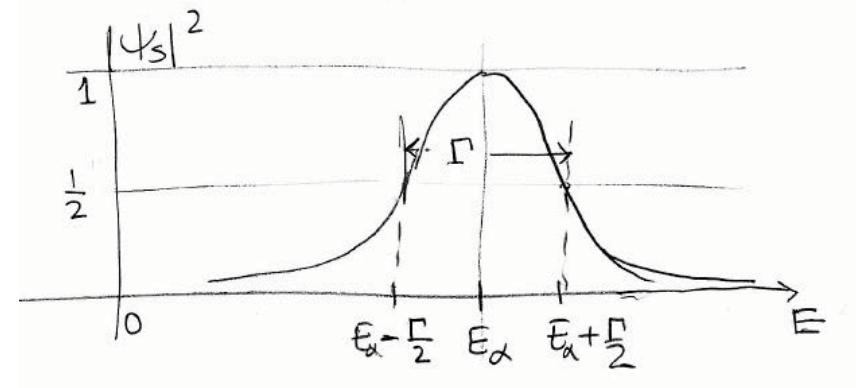
\includegraphics[width=0.5\linewidth]{resources/images/breit_wigner_distribution.png}
    \caption{A graph of the Breit-Wigner distribution. As shown, $\Gamma$ is the width at half maximum.}
    \label{breit_wigner_distribution}
\end{figure}

\subsection{Half-Width and Time Delay}\label{half_width_time_delay}

To better understand the significance of $\Gamma$, we define the associated time $\tau$, called the \textbf{lifetime} of the resonance: $$\tau=\frac{\hbar}{\Gamma}=\frac{m}{2\alpha\beta\hbar}.$$As you would expect, the lifetime is closely related to the time delay associated with a wavepacket at the resonant value $\alpha$ of $k$. We can evaluate this time delay: \begin{align*}\Delta t&=2\hbar\frac{d\delta}{dE}\\&=2\hbar\frac{dk}{dE}\frac{d\delta}{dk}\bigg|_{k=\alpha}\\&=\frac{2\hbar}{(\frac{\hbar^2k}{m})}(\frac{1}{\beta})\\&=\frac{2\hbar}{(\frac{\hbar^2\alpha\beta}{m})}\\&=\frac{2m}{\alpha\beta\hbar}=4\tau.\end{align*}Thus, the lifetime is simply one-fourth of the time delay.

\begin{framedrmk*}
    Unstable particles can be thought of as resonances. The Higgs boson, discovered in 2012, is an unstable particle with mass $E_\alpha=125$ GeV. It can decay into two photons, or into two taus, or into a $b\bar{b}$ pair, among others. The width $\Gamma$ associated with the Higgs is $4.07$ MeV $(\pm4\%)$. Its lifetime $\tau$ is about $1.62\times 10^{-22}$ seconds!
\end{framedrmk*}

\subsection{Resonances in the Complex $k$-Plane}\label{resonances_complex_plane}

We now try to understand resonances more mathematically. We saw that, at resonance, the norm of $A_s$ reaches a maximum value of $1$. Let's see what happens when $A_s$ is large. We have $$A_s=\sin\delta e^{i\delta}=\frac{\sin\delta}{e^{-i\delta}}=\frac{\sin\delta}{\cos\delta-i\sin\delta}=\frac{\tan\delta}{1-i\tan\delta}.$$At resonance, $\delta=\pi/2$ and $A_s=i$. On the other hand, if we \textit{really} want $A_s$ to be large, notice that $A_s$ becomes \textit{infinite} for $$\tan\delta=-i.$$This seems nonsensical! For the tangent of the phase shift to be complex, $\delta$  must also be complex, whatever that means. But let's think this through a bit more. Recall that near a resonance, $\tan\delta=\frac{\beta}{\alpha-k}.$ Then we have $$A_s=\frac{\frac{\beta}{\alpha-k}}{1-i\frac{\beta}{\alpha-k}}=\frac{\beta}{(\alpha-i\beta)-k}.$$At the resonant energy, $k=\alpha$, which gives $A_s=i$, as expected. If we instead think of the wavenumber $k$ as a \textit{complex} variable, we see that $A_s$ becomes infinite at $k=k_*=\alpha-i\beta$. (In complex analysis, this point is called a \textbf{pole}). This is the true location of the resonance! The real part is the resonant energy, and the imaginary part encodes the lifetime.

For small $\beta$, the resonance occurs near the real axis, as shown in Figure \ref{resonance_complex_plane}. As mentioned in Section \ref{modeling_a_resonance}, a smaller $\beta$ means a sharper resonance. As we can see, the value of $|A_s|$ on the real line becomes large for $k=\alpha$ because of its proximity to $k=k_*$. 

The lesson here is that we can search for resonances mathematically by solving for the complex $k$ values for which $$\boxed{\tan\delta(k)=-i.}$$The real parts of these $k$'s will be the resonant energies, and the imaginary parts will be the lifetimes.

The idea of a complex $k$ plane is very powerful. Suppose we consider purely imaginary values $k=i\kappa$, with $\kappa\in\mathbb{R}_+$. Then the energy takes the form $$E=-\frac{\hbar^2\kappa^2}{2m}<0,$$which can represent bound states. Indeed, one can plot the bound states in the complex $k$ plane along the positive imaginary axis, as shown in Figure \ref{resonance_complex_plane}. The complex $k$ plane has room to fit scattering states, resonances, and bound states!

\begin{figure}
    \centering
    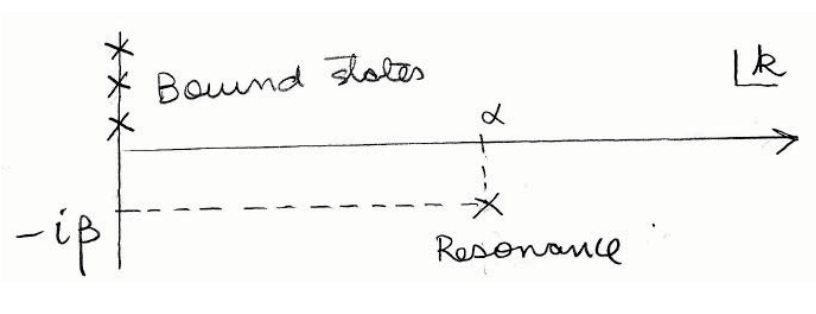
\includegraphics[width=0.5\linewidth]{resources/images/resonance_complex_plane.png}
    \caption{Resonances can be thought of as occurring for complex values of $k$, where the real part is the resonant energy and the imaginary part is the lifetime.}
    \label{resonance_complex_plane}
\end{figure}

\begin{framedrmk*}[Anti-bound states]
    Some physicists even include \textit{anti-bound states} on the \textit{negative} imaginary axis of the complex $k$ plane. While normal bound states are characterized by exponential decay in the classically forbidden region, anti-bound states are characterized by exponential \textit{increase} in this region. This may seem strange, but these states can actually be observed in nuclear physics, when a neutron is captured by some light nucleus.
\end{framedrmk*}
